\chapter{Peak Detector Figures \& Tables}\label{A:peak_detector}

\section*{Initial \& Final Peak Detector Output Comparison}\label{A:peak_detector_screenshots}

\subsection*{Peak Detector Output for a 150mV Peak to Peak Triangle Input}
\begin{figure}[H]
    
    \centering
    \begin{subfigure}{0.45\textwidth}
        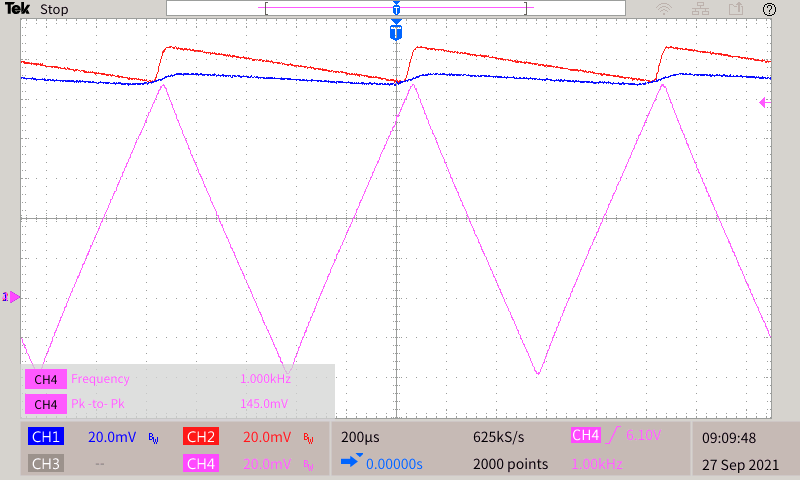
\includegraphics[width=\columnwidth]{current_sense/peak_comparison_150mV/1kHz_150mV.PNG}
        \subcaption{Initial (Red) \& final (Blue) peak detetor outputs for a 1$kHz$ triangle input.}
    \end{subfigure}
    \begin{subfigure}{0.45\textwidth}
        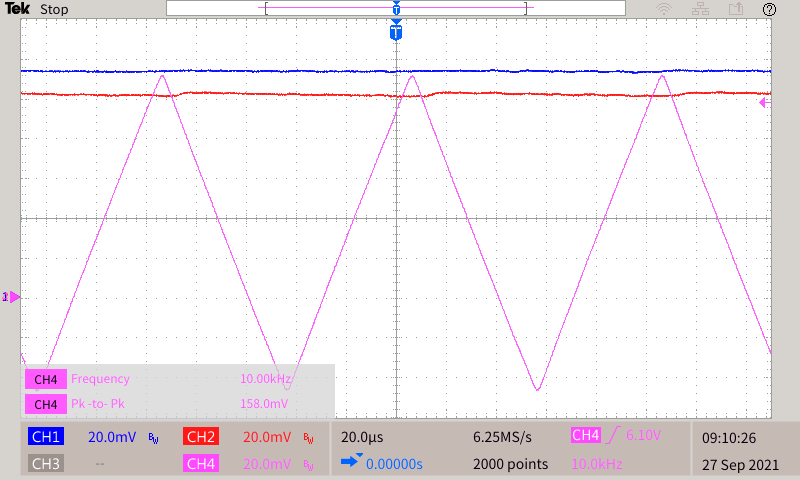
\includegraphics[width=\columnwidth]{current_sense/peak_comparison_150mV/10kHz_150mV.PNG}
        \subcaption{Initial (Red) \& final (Blue) peak detetor outputs for a 10$kHz$ triangle input.}
    \end{subfigure}
    \begin{subfigure}{0.45\textwidth}
        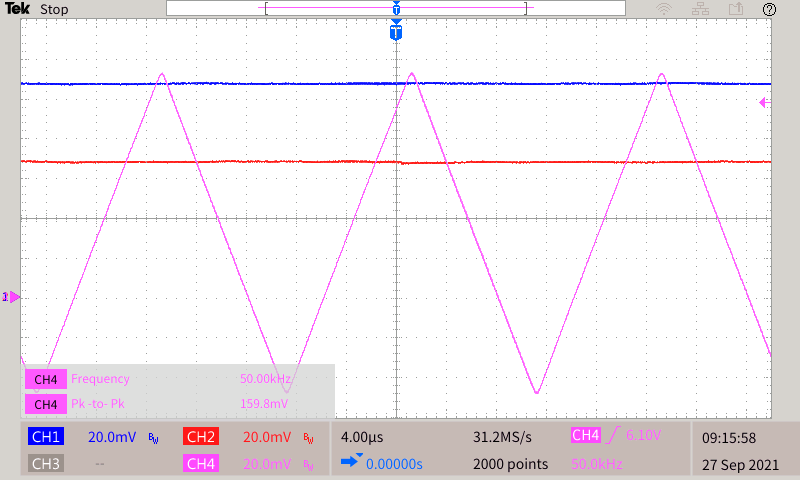
\includegraphics[width=\columnwidth]{current_sense/peak_comparison_150mV/50kHz_150mV.PNG}
        \subcaption{Initial (Red) \& final (Blue) peak detetor outputs for a 50$kHz$ triangle input.}
    \end{subfigure}
    \begin{subfigure}{0.45\textwidth}
        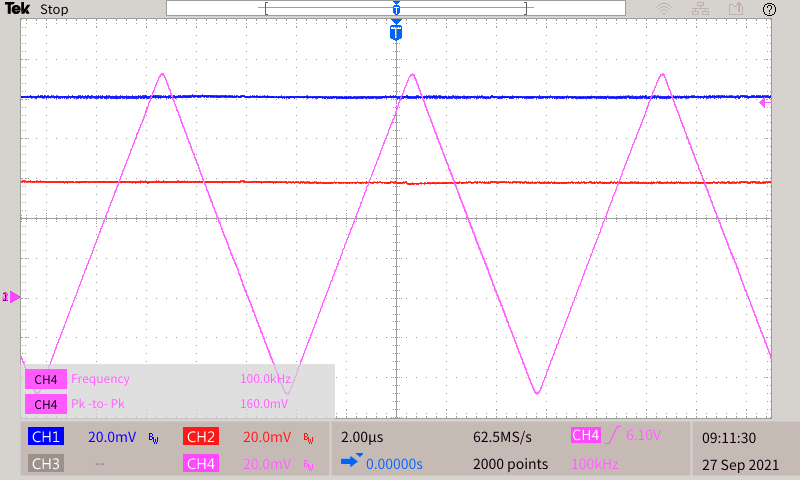
\includegraphics[width=\columnwidth]{current_sense/peak_comparison_150mV/100kHz_150mV.PNG}
        \subcaption{Initial (Red) \& final (Blue) peak detetor outputs for a 100$kHz$ triangle input.}
    \end{subfigure}
    \caption{Initial \& Final Peak Detector Output at varying frequencies for a 150mV peak to peak triangle input.}
\end{figure}

\subsection*{Peak Detector Output for a 500mV Peak to Peak Triangle Input}
\begin{figure}[H]
    
    \centering
    \begin{subfigure}{0.45\textwidth}
        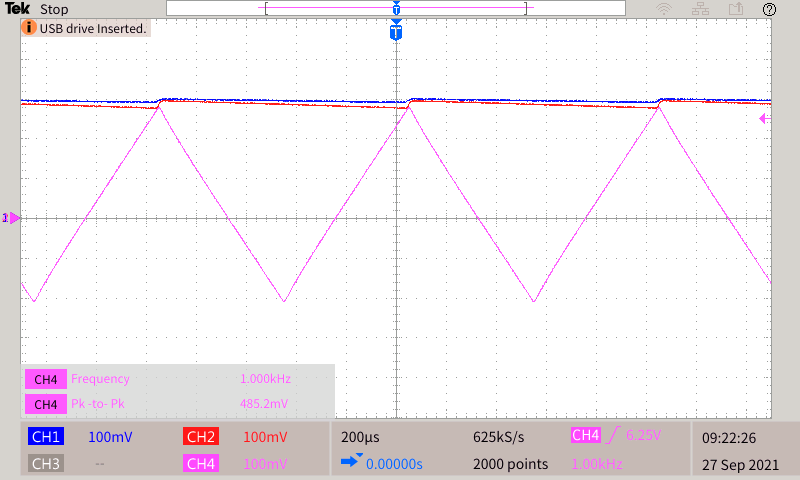
\includegraphics[width=\columnwidth]{current_sense/peak_comparison_500mV/1kHz_500mV.PNG}
        \subcaption{Initial (Red) \& final (Blue) peak detetor outputs for a 1$kHz$ triangle input.}
    \end{subfigure}
    \begin{subfigure}{0.45\textwidth}
        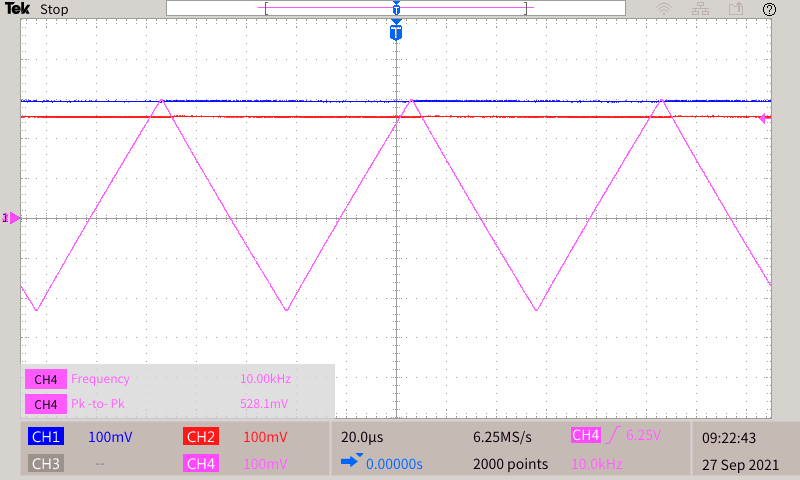
\includegraphics[width=\columnwidth]{current_sense/peak_comparison_500mV/10kHz_500mV.PNG}
        \subcaption{Initial (Red) \& final (Blue) peak detetor outputs for a 10$kHz$ triangle input.}
    \end{subfigure}
    \begin{subfigure}{0.45\textwidth}
        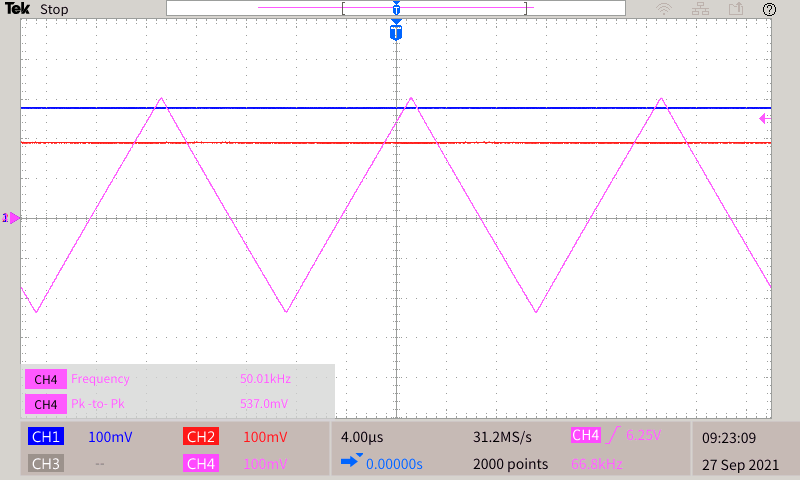
\includegraphics[width=\columnwidth]{current_sense/peak_comparison_500mV/50kHz_500mV.PNG}
        \subcaption{Initial (Red) \& final (Blue) peak detetor outputs for a 50$kHz$ triangle input.}
    \end{subfigure}
    \begin{subfigure}{0.45\textwidth}
        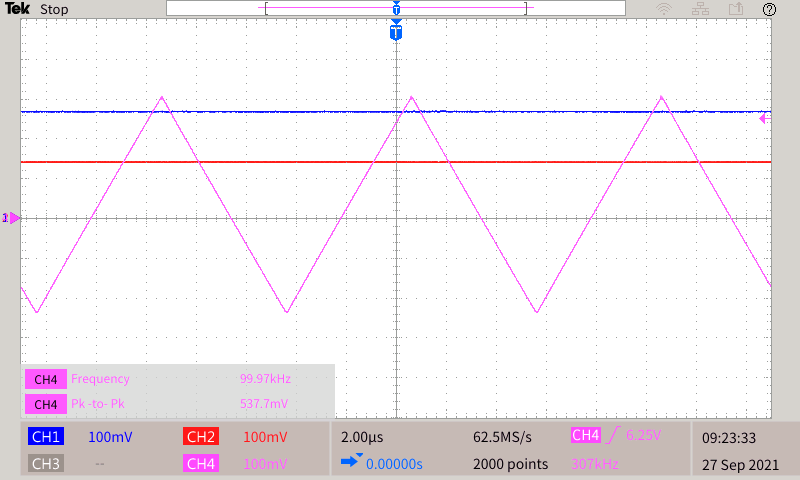
\includegraphics[width=\columnwidth]{current_sense/peak_comparison_500mV/100kHz_500mV.PNG}
        \subcaption{Initial (Red) \& final (Blue) peak detetor outputs for a 100$kHz$ triangle input.}
    \end{subfigure}
    \caption{Initial \& Final Peak Detector Output at varying frequencies for a 500mV peak to peak triangle input.}
\end{figure}

\subsection*{Peak Detector Output for a 1500mV Peak to Peak Triangle Input}
\begin{figure}[H]
    
    \centering
    \begin{subfigure}{0.45\textwidth}
        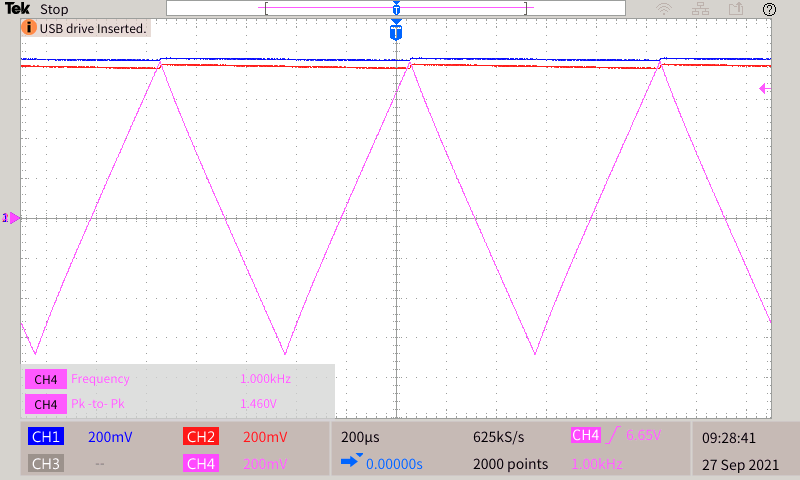
\includegraphics[width=\columnwidth]{current_sense/peak_comparison_1500mV/1kHz_1500mV.PNG}
        \subcaption{Initial (Red) \& final (Blue) peak detetor outputs for a 1$kHz$ triangle input.}
    \end{subfigure}
    \begin{subfigure}{0.45\textwidth}
        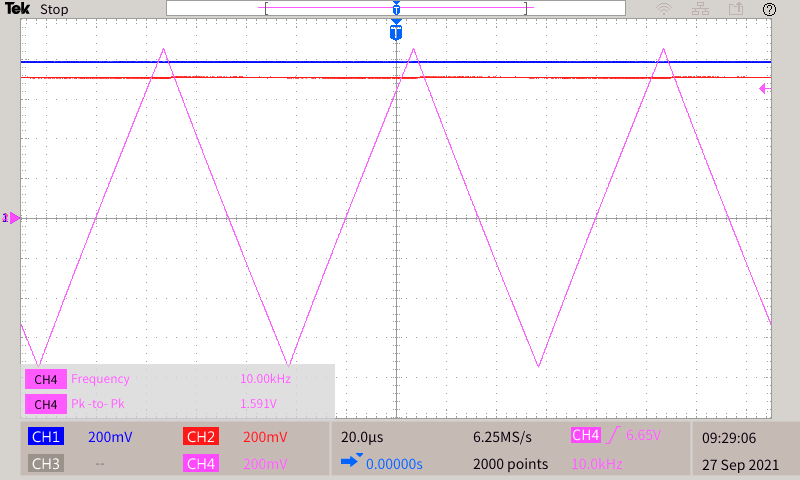
\includegraphics[width=\columnwidth]{current_sense/peak_comparison_1500mV/10kHz_1500mV.PNG}
        \subcaption{Initial (Red) \& final (Blue) peak detetor outputs for a 10$kHz$ triangle input.}
    \end{subfigure}
    \begin{subfigure}{0.45\textwidth}
        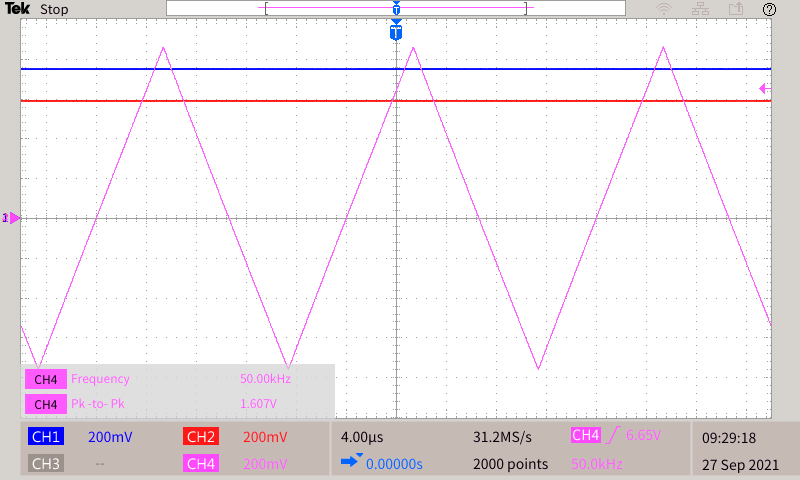
\includegraphics[width=\columnwidth]{current_sense/peak_comparison_1500mV/50kHz_1500mV.PNG}
        \subcaption{Initial (Red) \& final (Blue) peak detetor outputs for a 50$kHz$ triangle input.}
    \end{subfigure}
    \begin{subfigure}{0.45\textwidth}
        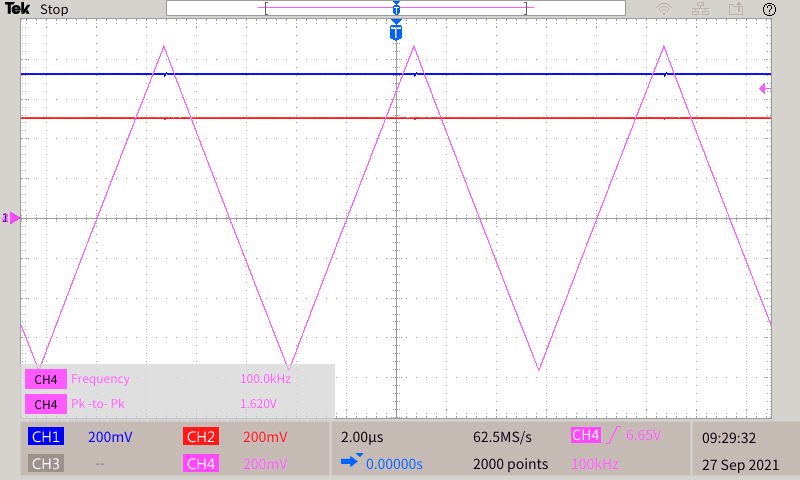
\includegraphics[width=\columnwidth]{current_sense/peak_comparison_1500mV/100kHz_1500mV.PNG}
        \subcaption{Initial (Red) \& final (Blue) peak detetor outputs for a 100$kHz$ triangle input.}
    \end{subfigure}
    \caption{Initial \& Final Peak Detector Output at varying frequencies for a 1500mV peak to peak triangle input.}
\end{figure}
    

\section*{Initial \& Final Peak Detector Output Error Plots}\label{A:peak_detector_plots}

\begin{figure}[H]
    \begin{center}
        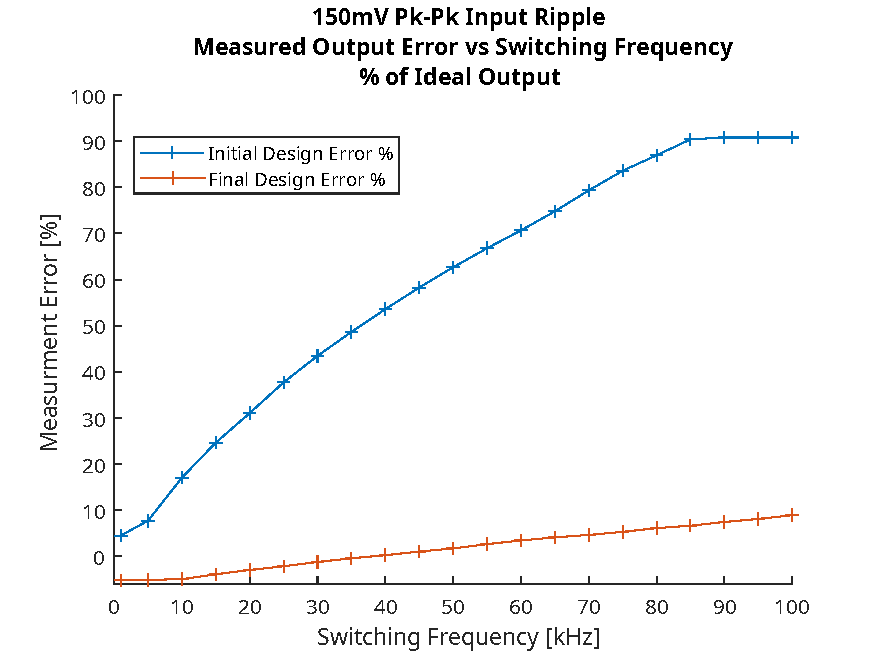
\includegraphics[width=0.8\textwidth]{current_sense/error/150mV_error.pdf}
        \caption{Initial \& final peak detector output error across frequencies for a 150mV peak to peak input. Displayed as a percentage of the ideal output.}
    \end{center}
\end{figure}

\begin{figure}[H]
    \begin{center}
        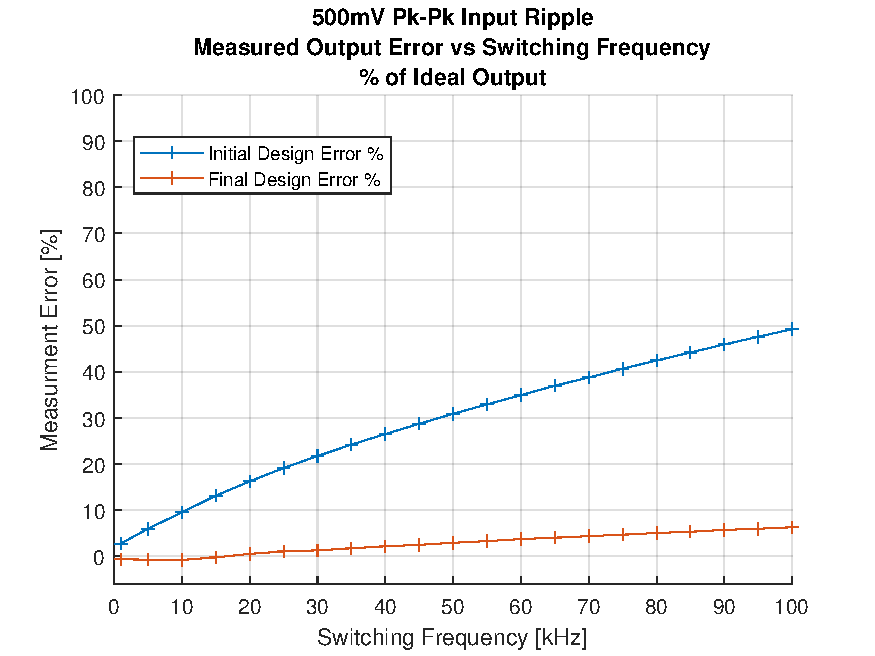
\includegraphics[width=0.8\textwidth]{current_sense/error/500mV_error.pdf}
        \caption{Initial \& final peak detector output error across frequencies for a 500mV peak to peak input. Displayed as a percentage of the ideal output.}
    \end{center}
    \vspace{-20pt}
\end{figure}

\begin{figure}[H]
    \begin{center}
        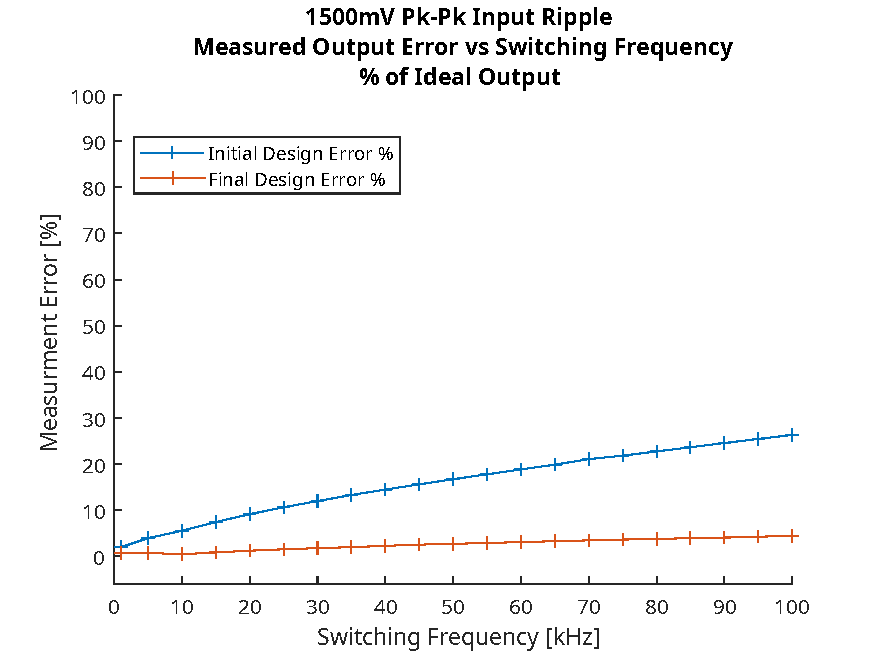
\includegraphics[width=0.8\textwidth]{current_sense/error/1500mV_error.pdf}
        \caption{Initial \& final peak detector output error across frequencies for a 1500mV peak to peak input. Displayed as a percentage of the ideal output.}
    \end{center}
\end{figure}


\newpage
\section*{Initial \& Final Peak Detector Output Error Tables}\label{A:peak_detector_tables}


\begin{table}[!ht]
    \centering
    \resizebox{\textwidth}{!}{%
        \begin{tabular}{|l|l|
                >{\columncolor[HTML]{DCFCDC}}l |l|
                >{\columncolor[HTML]{FCDADA}}l |}
            \hline
            \multicolumn{5}{|c|}{\cellcolor[HTML]{FFE4C3}\textbf{\begin{tabular}[c]{@{}c@{}}150mV  Peak to Peak Input Signal\\ Initial and Final Design Peak Detector Output Error Across Frequencies\end{tabular}}}                                                                                     \\ \hline
            \textbf{Frequency (kHz)} & \textbf{Final Design Error (mV)} & \textbf{Final Design \% Error} & \textbf{Initial Design Error (mV)} & \textbf{Initial Design \% Error} \\ \hline
            1                        & -3.90                            & -5.2                           & 3.40                               & 4.533333333                      \\ \hline
            5                        & -3.80                            & -5.066666667                   & 5.80                               & 7.733333333                      \\ \hline
            10                       & -3.70                            & -4.933333333                   & 12.80                              & 17.06666667                      \\ \hline
            15                       & -2.90                            & -3.866666667                   & 18.50                              & 24.66666667                      \\ \hline
            20                       & -2.20                            & -2.933333333                   & 23.30                              & 31.06666667                      \\ \hline
            25                       & -1.60                            & -2.133333333                   & 28.30                              & 37.73333333                      \\ \hline
            30                       & -0.90                            & -1.2                           & 32.60                              & 43.46666667                      \\ \hline
            35                       & -0.30                            & -0.4                           & 36.50                              & 48.66666667                      \\ \hline
            40                       & 0.20                             & 0.266666667                    & 40.20                              & 53.6                             \\ \hline
            45                       & 0.80                             & 1.066666667                    & 43.70                              & 58.26666667                      \\ \hline
            50                       & 1.30                             & 1.733333333                    & 47.00                              & 62.66666667                      \\ \hline
            55                       & 2.00                             & 2.666666667                    & 50.10                              & 66.8                             \\ \hline
            60                       & 2.60                             & 3.466666667                    & 53.00                              & 70.66666667                      \\ \hline
            65                       & 3.10                             & 4.133333333                    & 56.10                              & 74.8                             \\ \hline
            70                       & 3.50                             & 4.666666667                    & 59.50                              & 79.33333333                      \\ \hline
            75                       & 4.00                             & 5.333333333                    & 62.70                              & 83.6                             \\ \hline
            80                       & 4.60                             & 6.133333333                    & 65.20                              & 86.93333333                      \\ \hline
            85                       & 5.00                             & 6.666666667                    & 67.80                              & 90.4                             \\ \hline
            90                       & 5.60                             & 7.466666667                    & 68.10                              & 90.8                             \\ \hline
            95                       & 6.10                             & 8.133333333                    & 68.10                              & 90.8                             \\ \hline
            100                      & 6.70                             & 8.933333333                    & 68.10                              & 90.8                             \\ \hline
        \end{tabular}%
    }
    \caption{Table of output errors at varying frequencies for both the initial and final peak detection design with a 150mV peak to peak input signal.}
    \label{T:150mV_peak_error}
\end{table}


\begin{table}[!ht]
    \centering
    \resizebox{\textwidth}{!}{%
        \begin{tabular}{|l|l|
                >{\columncolor[HTML]{DCFCDC}}l |l|
                >{\columncolor[HTML]{FCDADA}}l |}
            \hline
            \multicolumn{5}{|c|}{\cellcolor[HTML]{FFE4C3}\textbf{\begin{tabular}[c]{@{}c@{}}500mV  Peak to Peak Input Signal\\ Initial and Final Design Peak Detector Output Error Across Frequencies\end{tabular}}}                                                                                     \\ \hline
            \textbf{Frequency (kHz)} & \textbf{Final Design Error (mV)} & \textbf{Final Design \% Error} & \textbf{Initial Design Error (mV)} & \textbf{Initial Design \% Error} \\ \hline
            1                        & -1.60                            & -0.64                          & 7.00                               & 2.8                              \\ \hline
            5                        & -1.70                            & -0.68                          & 15.00                              & 6                                \\ \hline
            10                       & -1.90                            & -0.76                          & 23.90                              & 9.56                             \\ \hline
            15                       & -0.50                            & -0.2                           & 32.90                              & 13.16                            \\ \hline
            20                       & 1.40                             & 0.56                           & 40.70                              & 16.28                            \\ \hline
            25                       & 2.70                             & 1.08                           & 47.90                              & 19.16                            \\ \hline
            30                       & 3.30                             & 1.32                           & 54.40                              & 21.76                            \\ \hline
            35                       & 4.40                             & 1.76                           & 60.60                              & 24.24                            \\ \hline
            40                       & 5.50                             & 2.2                            & 66.30                              & 26.52                            \\ \hline
            45                       & 6.30                             & 2.52                           & 71.90                              & 28.76                            \\ \hline
            50                       & 7.40                             & 2.96                           & 77.30                              & 30.92                            \\ \hline
            55                       & 8.30                             & 3.32                           & 82.40                              & 32.96                            \\ \hline
            60                       & 9.40                             & 3.76                           & 87.40                              & 34.96                            \\ \hline
            65                       & 10.20                            & 4.08                           & 92.50                              & 37                               \\ \hline
            70                       & 11.00                            & 4.4                            & 97.00                              & 38.8                             \\ \hline
            75                       & 11.80                            & 4.72                           & 101.70                             & 40.68                            \\ \hline
            80                       & 12.70                            & 5.08                           & 106.20                             & 42.48                            \\ \hline
            85                       & 13.40                            & 5.36                           & 110.50                             & 44.2                             \\ \hline
            90                       & 14.40                            & 5.76                           & 114.90                             & 45.96                            \\ \hline
            95                       & 15.00                            & 6                              & 119.00                             & 47.6                             \\ \hline
            100                      & 15.80                            & 6.32                           & 123.20                             & 49.28                            \\ \hline
        \end{tabular}%
    }
    \caption{Table of output errors at varying frequencies for both the initial and final peak detection design with a 500mV input signal.}
    \label{T:500mV_peak_error}
\end{table}


\begin{table}[!ht]
    \centering
    \resizebox{\textwidth}{!}{%
        \begin{tabular}{|l|l|
                >{\columncolor[HTML]{DCFCDC}}l |l|
                >{\columncolor[HTML]{FCDADA}}l |}
            \hline
            \multicolumn{5}{|c|}{\cellcolor[HTML]{FFE4C3}\textbf{\begin{tabular}[c]{@{}c@{}}1500mV  Peak to Peak Input Signal\\ Initial and Final Design Peak Detector Output Error Across Frequencies\end{tabular}}}                                                                                     \\ \hline
            \textbf{Frequency (kHz)} & \textbf{Final Design Error (mV)} & \textbf{Final Design \% Error} & \textbf{Initial Design Error (mV)} & \textbf{Initial Design \% Error} \\ \hline
            1                        & 5.40                             & 0.72                           & 15.00                              & 2                                \\ \hline
            5                        & 5.70                             & 0.76                           & 29.70                              & 3.96                             \\ \hline
            10                       & 3.60                             & 0.48                           & 41.70                              & 5.56                             \\ \hline
            15                       & 6.50                             & 0.866666667                    & 55.90                              & 7.453333333                      \\ \hline
            20                       & 9.40                             & 1.253333333                    & 68.70                              & 9.16                             \\ \hline
            25                       & 11.60                            & 1.546666667                    & 79.90                              & 10.65333333                      \\ \hline
            30                       & 13.50                            & 1.8                            & 90.00                              & 12                               \\ \hline
            35                       & 15.10                            & 2.013333333                    & 99.90                              & 13.32                            \\ \hline
            40                       & 17.20                            & 2.293333333                    & 108.70                             & 14.49333333                      \\ \hline
            45                       & 19.20                            & 2.56                           & 117.20                             & 15.62666667                      \\ \hline
            50                       & 20.50                            & 2.733333333                    & 125.50                             & 16.73333333                      \\ \hline
            55                       & 21.90                            & 2.92                           & 133.60                             & 17.81333333                      \\ \hline
            60                       & 23.30                            & 3.106666667                    & 141.50                             & 18.86666667                      \\ \hline
            65                       & 24.80                            & 3.306666667                    & 149.20                             & 19.89333333                      \\ \hline
            70                       & 26.10                            & 3.48                           & 158.20                             & 21.09333333                      \\ \hline
            75                       & 27.50                            & 3.666666667                    & 163.80                             & 21.84                            \\ \hline
            80                       & 28.60                            & 3.813333333                    & 170.70                             & 22.76                            \\ \hline
            85                       & 29.60                            & 3.946666667                    & 177.50                             & 23.66666667                      \\ \hline
            90                       & 30.70                            & 4.093333333                    & 184.40                             & 24.58666667                      \\ \hline
            95                       & 32.10                            & 4.28                           & 191.00                             & 25.46666667                      \\ \hline
            100                      & 33.40                            & 4.453333333                    & 197.50                             & 26.33333333                      \\ \hline
        \end{tabular}%
    }
    \caption{Table of output errors at varying frequencies for both the initial and final peak detection design with a 1500mV input signal.}
    \label{T:1500mV_peak_error}
\end{table}

